\section{StochasticEventGenerator Class Reference}
\label{classStochasticEventGenerator}\index{StochasticEventGenerator@{StochasticEventGenerator}}
Inheritance diagram for StochasticEventGenerator::\begin{figure}[H]
\begin{center}
\leavevmode
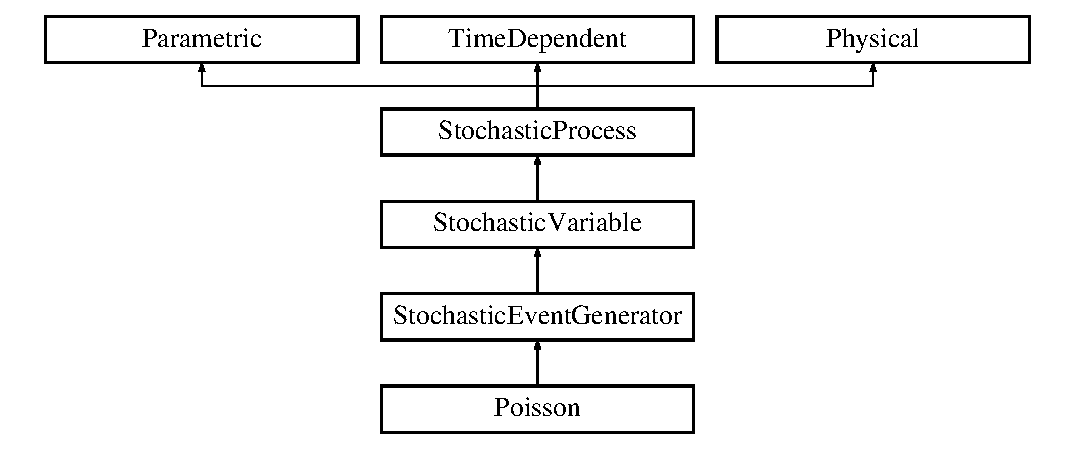
\includegraphics[height=5cm]{classStochasticEventGenerator}
\end{center}
\end{figure}


\subsection{Detailed Description}
An object which generates events. 

Useful for event-triggered averages. \subsection*{Public Member Functions}
\begin{CompactItemize}
\item 
{\bf StochasticEventGenerator} (class {\bf Time} $\ast$time, const string \&name=\char`\"{}\char`\"{}, const string \&type=\char`\"{}event\_\-generator\char`\"{})\label{classStochasticEventGenerator_f113f0914087df33485ec999204037c6}

\begin{CompactList}\small\item\em Create. \item\end{CompactList}\item 
virtual {\bf $\sim$StochasticEventGenerator} ()\label{classStochasticEventGenerator_fd363097980a3d600520e934b9fdfb1c}

\begin{CompactList}\small\item\em Destroy. \item\end{CompactList}\item 
virtual bool {\bf hasEvent} ()\label{classStochasticEventGenerator_25b18204e3b8f826ed0b0b5b9a4c755a}

\begin{CompactList}\small\item\em Whether an event is present. \item\end{CompactList}\end{CompactItemize}
